\section{Formal Methods and Verification}
%% TODO: varf�r �r formal methods i kursiv?
It is almost impossible to write specification in a natural language
and not make room for different interpretations and
misunderstandings. Hence \emph{Formal Methods} are introduced which
are based on formal languages that have precise rules. Describing a
system with formal notation gives the ability of automating test cases
for the system, since it is precisely defined.  Formal methods can be
used everywhere in the development life cycle and not only when
writing specification for the whole system.
\cite[p.272]{COURSEBOOK:safety-critical}

In the ISO standard ISO~26262, see section \ref{SEC:ISO26262},
something called semi-formal notation is also mentioned. The
difference being that formal notation needs both semantics and syntax
to be well defined but semi-formal notation needs only the definition
of semantics. \cite{ISO26262:car}

To determine whether the output of a life cycle phase fulfills the
requirements specified by a previous phase, \emph{verification} is
needed. Formal verification is the verification of a system
using formal methods.  The exact meaning of verification is however
confusing. The definition may differ in comparison
of academic or industrial use. Even in different phases of the safety
life cycle verification is conducted in various forms.
\cite{thomas_arts}\cite[8:9.2]{ISO26262}\cite[p.309]{COURSEBOOK:safety-critical}

\section{Industrial Standards}

\subsection {IEC~61508 and ISO~26262}
\label{SEC:ISO26262}
IEC 61508 adopts a four level system for categorizing the severity of
hazards. It also adopts a six level system for classifying the
frequency of a hazard. There are four risk classes which are given the
values 1-4 where 1 corresponds to the most serious accidents and 4 to
the least serious. Based on this, IEC 61508 has a four level
classification of safety integrity levels called SIL, ranged from 1,
being the least critical, to 4, being the most critical. Each of the
safety integrity levels has a criteria of maximum frequency of
failures which a system built on that SIL must satisfy. In other
words, a SIL is a level of measure of the reliability of a safety
function.  Due to the fact that the failure of a safety function can
lead to a hazardous event, the safety integrity of a specific safety
function must be of such a level to ensure that the failure frequency
is sufficiently low or that the consequences of the hazardous event
are modified to meet a tolerable risk. To ensure safety, functions
with SIL 4 need to be tested and documented the most.
\cite{COURSEBOOK:safety-critical}\cite{IEC61508}\cite{Advances:IEC61508}\cite{Advances:SIL4}

The automotive functional safety standard, ISO~26262, has adopted a
similar system of safety integrity levels, called automotive safety
integrity levels or ASIL. As with IEC~61508 there are four integrity
levels, ranged A-D, but there are no direct correlation between the
two. \cite{TI:safety_critical}

ISO~26262 describes the full development process, from concept to
production, with functional safety in mind. For software development,
the standard has a reference model with different phases of the
process, see figure~\ref{FIG:ISO:phases}. Each phase in the reference
model is dependent on the earlier phases. The reference model has the
shape of a V, where the left side contains all development phases, and
the right side contains the test phases. The work flow from this view
starts with the phase ``specification of software safety
requirements''. This phase specifies the software requirements needed
to ensure the stability of the system. They are derived from the
system design specification. This is part of the integration between
software and hardware. The second phase is the ``software
architectural design''. It represent the interaction between all
software components. The third phase and the last development phase,
in the model is the ``software unit design and implementation''. This
phase contains the implementation of each module. If the
implementation does not meet the specified safety, the product needs
to go back to an earlier phase and be redesigned. \cite[6:5.4]{ISO26262}\cite[p.8-9]{COURSEBOOK:safety-critical}

\begin{figure}
  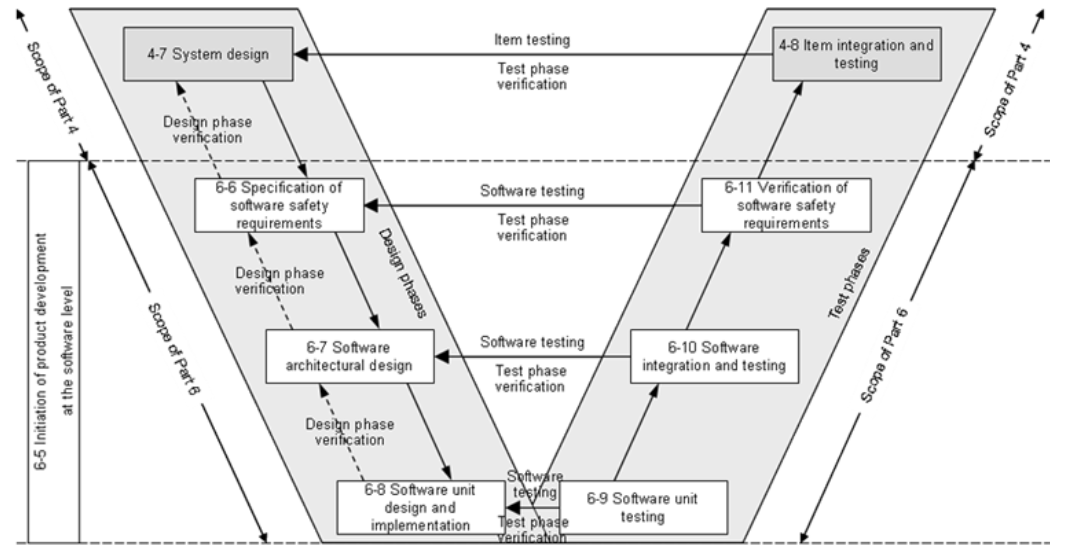
\includegraphics[keepaspectratio, width=\linewidth]{pictures/V}
  \caption{Phases of software development in the standard ISO~26262}
  \label{FIG:ISO:phases}
\end{figure}

Each of these phases is tested thoroughly with the phases ``software
unit testing'', ``software integration and testing'' and
``verification of software safety requirements''. The unit testing
phase confirms that the implementation of the module fulfills the
design specifications. If the product pass this phase, it continues to
the integration and testing phase, otherwise it is sent back to the
implementation phase. The objective in the phase software integration
and testing is to integrate the software units and demonstrate that
the architectural design is correct. A demonstration that the software
safety requirements is meet, is performed in the phase ``verification
of software safety requirements''. \cite[6:5.4]{ISO26262}

\subsection{AUTOSAR (AUTomotive Open System ARchitecture)}
The AUTOSAR platform has a layered software architecture. This means
that the architecture is divided to a number of different layers, such
as the application layer, runtime environment, the basic software
layer, and the microcontroller. In the
figure~\ref{FIG:AUTOSAR:architecture} the basic software layer is
represented as four different parts; services, ECU abstraction,
microcontroller abstraction, and complex
drivers. \cite{AUTOSAR:LayeredSoftwareArchitecture}

\begin{figure}[!ht]
  \begin{center}
    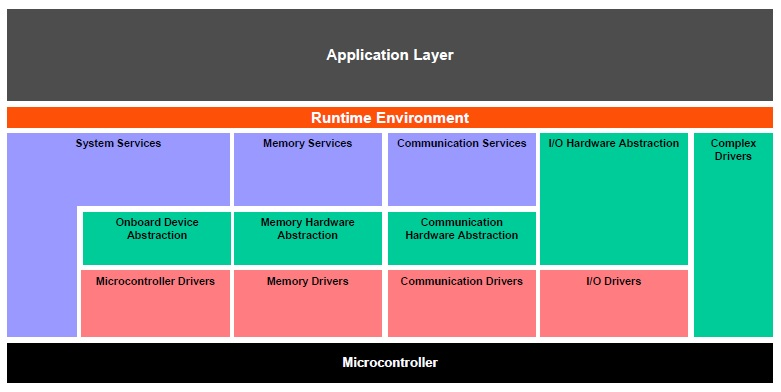
\includegraphics[keepaspectratio, width=\linewidth]{pictures/autosar_architecture.jpg}
  \end{center}
  \caption{The AUTOSAR software architecture. Noticeable is that the basic
    software layer is divided further into four categories with even more subsections.}
  \label{FIG:AUTOSAR:architecture}
\end{figure}

%% TODO: vad menas med "onboard device abstraction"?
The runtime environment is the operating system, and the
microcontroller is the hardware. The software running in the
application layer are for example software components for sensors and
actuators. One example of how the different parts in the basic
software layer is integrated, is the watchdog, which consist of
several parts as seen in figure~\ref{FIG:AUTOSAR:watchdog}. The
microcontroller abstraction layer has the drivers for the watchdog;
the interaction with the microcontroller. Then there is the watchdog
interface at the ECU abstraction layer. The watchdog interface is the
onboard device abstraction. Last is the watchdog manager (abbreviated
WdgM) which runs as a system service in the service layer. \cite{AUTOSAR:LayeredSoftwareArchitecture}

\begin{figure}[!ht]
  \begin{center}
    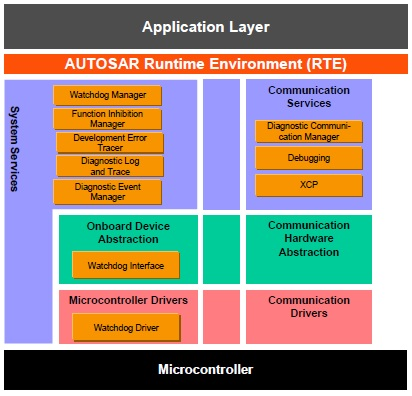
\includegraphics{pictures/watchdog_architecture.jpg}
  \end{center}
  \caption{The Watchdog and some other related modules.}
  \label{FIG:AUTOSAR:watchdog}
\end{figure}

The watchdog have a number of dependencies to other services in the
basic software layer. For example when an error is found by the
watchdog, it could either be reported to the diagnostic event manager
or the development error tracer depending on the type of error. These
are two services that are used for error management. \cite{SPEC:AUTOSAR:WDGM}

AUTOSAR's concept is to make it possible for vehicle manufacturers to
buy modules from different software developers, which will still work
together in unison. For a software developer to present a software
module with functionality that fits different vehicle manufacturers,
the standard introduces configurations. The configurations specifies a
number of parameters that can be configured in order to fit a specific
vehicle manufacture. In the watchdog manager for example, there is
parameters that specify if the watchdog manager should report errors
to the diagnostic event manager (DEM), or which type of supervision
that should be executed and what to supervise. \cite{AUTOSAR:basic_info}\cite{AUTOSAR:LayeredSoftwareArchitecture}

The current version of AUTOSAR, version 4, has been design with
functional safety in mind. Essential concepts of ISO~26262 have been
developed alongside AUTOSAR. \cite{AUTOSAR:basic_info}

\section{Verification Methods}
The standard IEC~61508 propose two methods to formal verify a
program. The key is to model the program into one of the following
state transition models. \cite[p. 127]{IEC61508}

\begin{enumerate}
\item \label{enum:FSM} Finite state machines/state transition diagrams
\item Time Petri nets
\end{enumerate}

IEC~61508 emphasises that Time Petri nets are best suited for
concurrent programs. Regarding the finite state machine method, the
following criteria needs to be satisfied for the implemented state
machine to be formal verified \cite[p. 77-79]{IEC61508}\cite[p. 322]{COURSEBOOK:safety-critical}:

\begin{description}
  \item[completeness] the system must have an action and new state for
    every input in every state,
  \item[consistency] only one state change is described for each
    state/input pair, and
  \item[reachability] whether or not it is possible to get from one
    state to another by any sequence of inputs.
\end{description}

%% TODO: Referenser
If the state machine is correctly implemented it represents a correct
model of the original program. If it does not exist any unwanted
transitions or states, then the original program is formal verified.

Since most program specifications are written in natural languages
there may be lot of ambiguities. Techniques have been developed to
reduce such cases, and these techniques are often referred to as semi
formal verification, because they often lack the mathematical rigor
associated with formal verification. These methods use textual,
graphical or other notation; often several techniques are used in
unity. \cite[p. 91]{COURSEBOOK:safety-critical}

The description of semi formal verification in IEC~61508 states:
''Semi-formal methods provide a means of developing a description of a
system at some stage in its development, i.e. specification, design or
coding. The description can in some cases be analyzed by machine or
animated to display various aspects of the system behavior.'' \cite[p. 77]{IEC61508}


\subsection{QuickCheck}
%% TODO: dubbelkolla sista meningen, r�cker med att ha byte koden + bibliotek?
QuickCheck was invented by Koen Claessen and John Hughes, as a testing
module for Haskell in 2000. In 2006 John Hughes founded the company
Quviq together with Thomas Arts \cite{QUVIQ:about}. Quviq offers a
commercial version of QuickCheck for Erlang. The main difference,
except from the programming language, is that the commercial version
of QuickCheck has a C-testing interface. Hence it possible to test
C-code in Erlang with the help of QuickCheck. All test code is written
in Erlang and checked against API calls to the C-code. It is not
necessary to have the actual source code; it is enough to only have
the compiled byte code and some library files of the program to test.

QuickCheck tests a program that has its specification implemented as
properties that must hold for the program
\cite{QUICKCHECK:manual}. QuickCheck provides guided random test
generation. This means that the samples can be weighted to cover
certain parts of the state-space with more likelihood.
